\documentclass[journal]{IEEEtran}
\usepackage[a5paper, margin=10mm]{geometry}
%\usepackage{lmodern} % Ensure lmodern is loaded for pdflatex
\usepackage{tfrupee} % Include tfrupee package


\setlength{\headheight}{1cm} % Set the height of the header box
\setlength{\headsep}{0mm}     % Set the distance between the header box and the top of the text


%\usepackage[a5paper, top=10mm, bottom=10mm, left=10mm, right=10mm]{geometry}

%
\setlength{\intextsep}{10pt} % Space between text and floats

\makeindex


\usepackage{cite}
\usepackage{amsmath,amssymb,amsfonts,amsthm}
\usepackage{algorithmic}
\usepackage{graphicx}
\usepackage{textcomp}
\usepackage{xcolor}
\usepackage{txfonts}
\usepackage{listings}
\usepackage{enumitem}
\usepackage{mathtools}
\usepackage{gensymb}
\usepackage{comment}
\usepackage[breaklinks=true]{hyperref}
\usepackage{tkz-euclide} 
\usepackage{listings}
\usepackage{multicol}
\usepackage{xparse}
\usepackage{gvv}
%\def\inputGnumericTable{}                                 
\usepackage[latin1]{inputenc}                                
\usepackage{color}                                            
\usepackage{array}                                            
\usepackage{longtable}                                       
\usepackage{calc}                                             
\usepackage{multirow}                                         
\usepackage{hhline}                                           
\usepackage{ifthen}                                               
\usepackage{lscape}
\usepackage{tabularx}
\usepackage{array}
\usepackage{float}
\usepackage{ar}
\usepackage[version=4]{mhchem}


\newtheorem{theorem}{Theorem}[section]
\newtheorem{problem}{Problem}
\newtheorem{proposition}{Proposition}[section]
\newtheorem{lemma}{Lemma}[section]
\newtheorem{corollary}[theorem]{Corollary}
\newtheorem{example}{Example}[section]
\newtheorem{definition}[problem]{Definition}
\newcommand{\BEQA}{\begin{eqnarray}}
\newcommand{\EEQA}{\end{eqnarray}}

\theoremstyle{remark}


\begin{document}
\bibliographystyle{IEEEtran}
\onecolumn

\title{METALLURGY ENGINEERING}
\author{GATE 2009\\
EE25BTECH11027-INDHIRESH S}
\maketitle


\renewcommand{\thefigure}{\theenumi}
\renewcommand{\thetable}{\theenumi}

\section{Q1 - Q20 carry one mark each}
\begin{enumerate}
\item  In a $n\times n $ identity matrix, the trace equals: \hfill{\brak{\text{GATE MT 2009}}}

\begin{multicols}{4}
\begin{enumerate}
\item $0$
\item $1$
\item $n$
\item $n^2$
\end{enumerate}
\end{multicols}

\item  Gibbs free energies of a system in states $1$ and $2$ are denoted by $G_1$ and $G_2$ respectively. The system will go spontaneously from state $1$ to state $2$ , if and only if: \hfill{\brak{\text{GATE MT 2009}}}
\begin{multicols}{4}
\begin{enumerate}
\item $G1-G2>0$
\item $G1-G2<0$
\item $G1-G2=0$
\item $G1<0 , G2<0$
\end{enumerate}
\end{multicols}

\item Flux in welding process acts as:
\hfill{\brak{\text{GATE MT 2009}}}
\begin{multicols}{2}
\begin{enumerate}
\item catalyst
\item protective agent
\item filler
\item heat generator
\end{enumerate}
\end{multicols}

\item  In an ideal HCP packing , the $\frac{c}{a}$ ratio is:\hfill{\brak{\text{GATE MT 2009}}}

\begin{multicols}{4}
\begin{enumerate}
\item $1.225$
\item $1.414$
\item $1.633$
\item $1.732$
\end{enumerate}
\end{multicols}

\item  A property that CANNOT be obtained from a tensile test is
\hfill{\brak{\text{GATE MT 2009}}}
\begin{multicols}{2}
\begin{enumerate}
\item Young's modulus
\item yield strength
\item ultimate tensile strength
\item endurance limit
\end{enumerate}
\end{multicols}

\item  Intensive thermodynamic variables are \hfill{\brak{\text{GATE MT 2009}}}
\begin{enumerate}
\item independent of the number of moles in the system
\item dependent on the volume of the system
\item dependent on the volume of the system
\item dependent on the volume of the system
\end{enumerate}

\item In a sound casting , the last liquid to solidify is in the \hfill{\brak{\text{GATE MT 2009}}}
\begin{multicols}{4}
\begin{enumerate}
\item runner
\item riser
\item gate
\item vent
\end{enumerate}
\end{multicols}

\item An annealed plain carbon steel, showing fully pearlitic microstructure , has a carbon content of\hfill{\brak{\text{GATE MT 2009}}}
\begin{multicols}{4}
\begin{enumerate}
\item $0.001wt\%$
\item $0.20wt\%$
\item $0.77wt\%$
\item $1.20wt\%$
\end{enumerate}
\end{multicols}

\item Superalloys are \hfill{\brak{\text{GATE MT 2009}}}
\begin{multicols}{2}
\begin{enumerate}
\item Al-based alloys
\item Cu-based alloys
\item Ni-based alloys
\item Mg-based alloys
\end{enumerate}
\end{multicols}

\item Wood is naturally occurring 
\hfill{\brak{\text{GATE MT 2009}}}
\begin{multicols}{2}
\begin{enumerate}
\item malleable material
\item composite material
\item ceramic material
\item isotropic material    
\end{enumerate}
\end{multicols}
\item The function, $f(x)=ax^2+bx+c$ has a maximum only if \hfill{\brak{\text{GATE MT 2009}}}
\begin{multicols}{4}
\begin{enumerate}
        \item$a<o$
        \item $a>0$
        \item $a=0$
        \item $a>0\;\text{and}\;b<0$
\end{enumerate}
\end{multicols}
\item A furnace wall consists of four layers of different materials $M1,M2,M3 \;      \text{and}\; M4$. If the layers are of equal thickness and the steady state temperature profile is, as shown below , then the material with the lowest thermal conductivity is\hfill{\brak{\text{GATE MT 2009}}}
\begin{figure}[H]
    \centering
    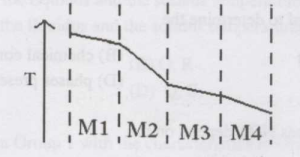
\includegraphics[width=0.5\linewidth]{figs/Q.12.png}
    \caption\centering{STUDY STATE TEMPERATURE PROFILE}
    \label{fig:placeholder}
\end{figure}
\begin{multicols}{4}
\begin{enumerate}
    \item $M1$
    \item $M2$
    \item $M3$
    \item $M4$
\end{enumerate}
\end{multicols}
\item From the list given below 
\begin{enumerate}[label=\Alph*),start = 16]
    \item Cu
    \item Mg
    \item Ni
    \item Zn
\end{enumerate}
two metals which provide cathodic protection to steel are\hfill{\brak{\text{GATE MT 2009}}}
\begin{multicols}{4}
\begin{enumerate}
    \item P,R
    \item R,S
    \item Q,R
    \item Q,S
\end{enumerate}
    
\end{multicols}


\item The Miller indices of the plane PQRS, shown in the unit cell are\hfill{\brak{\text{GATE MT 2009}}}
\begin{figure}[H]
    \centering
    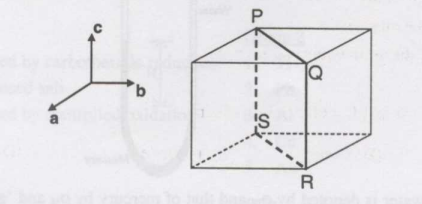
\includegraphics[width=0.5\textwidth]{figs/Q.14.png}
    \caption\centering{THE UNIT CELL}
    \label{fig:placeholder}
\end{figure}
\begin{multicols}{4}
\begin{enumerate}
\item $111$
\item$121$
\item $110$
\item $100$
\end{enumerate}
\end{multicols}

\item A defect that is bounded by two mirror plane is
\hfill{\brak{\text{GATE MT 2009}}}
\begin{multicols}{4}
\begin{enumerate}
\item twin
\item stacking fault
\item grain boundry
\item edge dislocation
\end{enumerate}
\end{multicols}

\item  $\lim_{x \to 0} \frac{sinx}{x}$ is equal to\hfill{\brak{\text{GATE MT 2009}}}

\begin {multicols}{4}
\begin{enumerate}
\item $0$
\item $1$
\item $\infty$
\item undefined
\end{enumerate}
\end{multicols}

\item  Fick's first law relates
\hfill{\brak{\text{GATE MT 2009}}}
\begin{enumerate}
\item flux of atoms and the concentration gradient
\item amount of gas dissolved in the molten metal and the partial pressure
\item applied normal stress and the orientation of slip system
\item heat flux and the temperature gradient
\end{enumerate}

\item  X-ray radiography is used to determine the \hfill{\brak{\text{GATE MT 2009}}}
\begin{multicols}{2}
\begin{enumerate}
\item soundness of casting
\item chemical composition
\item crystal structure
\item phase present
\end{enumerate}
\end{multicols}

\item Hardenability of steel does NOT depend on the\hfill{\brak{\text{GATE MT 2009}}}
\begin{multicols}{2}
\begin{enumerate}
\item alloy content
\item grain size
\item amount of carbon present
\item amount of cold work
\end{enumerate}
\end{multicols}

\item p-type semiconductor can be obtained by doping silicon with\hfill{\brak{\text{GATE MT 2009}}}
\begin{multicols}{4}
\begin{enumerate}
\item antimony
\item phosphorous
\item arsenic
\item boron
\end{enumerate}
\end{multicols}

\section{Q21 - Q60 carry 2 marks each}
\item The figure below shows water over mercury manometer. if the density of water is denoted by $\rho_w$ and that of mercury by $\rho_M$ and $'g'$ denotes the acceleration due to gravity , the pressure difference $(P_A - P_B)$ will be equal to\hfill{\brak{\text{GATE MT 2009}}}
\begin{figure}[H]
    \centering
    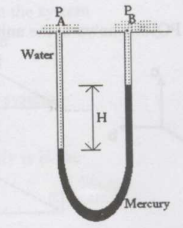
\includegraphics[width=0.2\textwidth]{figs/Q.21.png}
    \caption\centering{MERCURY MANOMETER}
    \label{fig:placeholder}
\end{figure}
\begin{multicols}{4}
\begin{enumerate}
    \item $-(\rho_M gH)$
    \item ($ \rho_W  -\rho_M$)gH
    \item  $rho_M$gH
    \item ($\rho_M-\rho_W$)gH
\end{enumerate}
\end{multicols}
\item Match the processes given in Group 1 with the coresponding typical defects given in group 2\hfill{\brak{\text{GATE MT 2009}}}\\
\begin{center}
\begin{tabular}{c c}
 
Group 1 & Group 2 \\ 
P.Forging & 1. Alligatoring\\
Q.Rolling & 2.Cold shut\\
R.Deep drawing & 3.Chevron cracks\\
S.Extrusion &  4. wrinkles
\end{tabular}
\end{center}
\begin{multicols}{2}
\begin{enumerate}
    \item$ P-1,Q-2,R-3,S-4$
    \item$P-2,Q-1,R-4,S-3$
    \item $P-2,Q-1,R-3,S-4$
    \item $P-3,Q-1,R-4,S-2$
\end{enumerate}
\end{multicols}
\item From the list given below , two factors that promotes coring in cast alloys are   \hfill{\brak{\text{GATE MT 2009}}}
\begin{enumerate}[label=\Alph*),start=16] 

    \item slow cooling during solidification  
    \item rapid cooling during solidification
    \item small difference between the liquids and solidus temperatures
    \item large difference between the liquidus and solidus temperatures
\end{enumerate}
\begin{multicols}{4}
\begin{enumerate}
    \item P,R
    \item Q,R
    \item P,S
    \item Q,S
\end{enumerate}
\end{multicols}
\item Match the loading conditions in group 1 with the characteristics in group 2.\hfill{\brak{\text{GATE MT 2009}}}
\begin{center}
\begin{tabular}{c c}
Group 1     &Group2  \\
P.Tensile     &1.barreling\\
Q.Compressive &2. Intergranular cracking\\
R.Fatigue &3. striations\\
S.Creep &4.Cup and cone\\
       &5.Earing
\end{tabular}
\end{center}
\begin{multicols}{2}
\begin{enumerate}
    \item $P-4,Q-5,R-3,S-1$
    \item $P-4,Q-1,R-3,S-2$
    \item $P-5,Q-1,R-4,S-2$
    \item $P-1,Q-2,R-3,S-5$
\end{enumerate}
\end{multicols}
\item  Match the extraction methods in group 1 with the metals in group 2 \hfill{\brak{\text{GATE MT 2009}}}
\begin{center}
\begin{tabular}{c c}
Group 1     &Group 2  \\
P. roasting followed by carbothermic reduction     & 1. Ti\\
Q. electrolysis of fused salt & 2.Pb\\
R. roasting followed by controoled oxidation & 3.Al\\
S. halide process & 4. Cu\\
      &5. Au
\end{tabular}
\end{center}

\begin{multicols}{2}
\begin{enumerate}
\item $P-2,Q-3,R-4,S-1$
\item $P-5,Q-4,R-3,S-1$
\item $P-2,Q-5,R-1,S-4$
\item $P-3,Q-2,R-5,S-1$
\end{enumerate}
\end{multicols}

\item  The average molecular weight of high density polyethylene is found to be $56000$.The degree of polymerization is \hfill{\brak{\text{GATE MT 2009}}}
\begin{multicols}{4}
\begin{enumerate}
\item $200$
\item $1000$
\item $2000$
\item $4000$
\end{enumerate}
\end{multicols}

\item A $0.2wt\%$ C steel is carburized at $1200K$ for $4$ hours to obtain $0.8wt\%$ at a depth of $0.20mm$ . Instead , if the carburizing is performed for $8$ hours at the same temperature , then $0.8wt\%$ C will be acheived at a depth of
\hfill{\brak{\text{GATE MT 2009}}}
\begin{multicols}{4}
\begin{enumerate}
\item $0.23mm$
\item $0.55mm$
\item $0.28mm$
\item $0.40mm$
\end{enumerate}
\end{multicols}

\item  A unit dislocation with a Burgers vector $\vec{b_1}$ will dissociate into two partial dislocations with burgers vectors $\vec{b_2}$ and $\vec{b_3}$ , if and only if  \hfill{\brak{\text{GATE MT 2009}}}
\begin{enumerate}[label=\Alph*),start=16] 
    \item  $\vec{b_1^2}$ $>$ $\vec{b_2^2} + \vec{b_3^2}$
    \item  $\vec{b_1^2}$ $<$ $\vec{b_2^2} + \vec{b_3^2}$
    \item  $\vec{b_1^2}$ $=$ $\vec{b_2^2} + \vec{b_3^2}$
    \item  $\vec{b_1^2}$ $\neq$ $\vec{b_2^2} + \vec{b_3^2}$
\end{enumerate}
\begin {multicols}{4}
\begin{enumerate}
\item P,R
\item P,S
\item Q,R
\item Q,S
\end{enumerate}
\end{multicols}

\item The solution function $y=f(x)$ for the ordinary differential equation, $\frac{dy}{dx} = 3x^2 - 2x$, passes through $(1,1)$. The magnitude of y at $x=3 $ is
\hfill{\brak{\text{GATE MT 2009}}}
\begin{multicols}{4}
\begin{enumerate}
\item $0$
\item $18$
\item $19$
\item $21$
\end{enumerate}
\end{multicols}

\item What is the magnitude of the following integral using single step application of trapezoid rule?\hfill{\brak{\text{GATE MT 2009}}}
\begin{align}
 \int_0^2(3x^2 + 4x  -2)dx
\end{align}
\begin{multicols}{4}
\begin{enumerate}
\item $9$
\item $16$
\item $18$
\item $36$
\end{enumerate}
\end{multicols}

\item During a sheet stamping operation, it is observed that sheet surface area triples . the true thickness strain is  \hfill{\brak{\text{GATE MT 2009}}}
\begin{multicols}{4}
\begin{enumerate}
\item $-1.1$
\item $-0.333$
\item $+0.333$
\item $+1.1$
\end{enumerate}
\end{multicols}
\item Match the practices in Group 1 with reactors in Group 2.\hfill{\brak{\text{GATE MT 2009}}}
\begin{center}
\begin{tabular}{c c}
Group 1     &  Group 2\\
P. Layered charging of coke and ore     &1. Ladle furnace\\
Q. Oxygen injection through supersonic nozzle &2. Electric arc furnace\\ 
R. Aluminium wire feeding &3. Blast furnace\\
S.Foamy slag practice & 4.LD converter
\end{tabular}
\end{center}
\begin{multicols}{2}
\begin{enumerate}
\item P-3,Q-1,R-2,S-4
\item P-2,Q-4,R-3,S-1
\item P-4,Q-3,R-2,S-1
\item P-3,Q-4,R-1,S-2
\end{enumerate}
\end{multicols}

\item For the reaction,\\
\begin{center}
    
$MO(Pure, Solid) + CO(gas) \longrightarrow M(Pure, Solid) + CO_2 (gas)$
\end{center}
the equilibrium constant at $1000K$ is $2.0$. The oxide, MO, can be reduced to M at $1000K$, using a gas
mixture containing
\hfill{\brak{\text{GATE MT 2009}}}
\begin{multicols}{2}
\begin{enumerate}
\item $20\% CO , 45\% CO_2, 35\% N_2$
\item  $20\% CO, 10\% CO_2, 70\% N_2$
\item$20\% O_2, 80\% N_2$
\item $50\% N_2, 50\%Ar$
\end{enumerate}
\end{multicols}

\item  Stacking fault energy (SFE) plays an important role in determining the work hardening ability of a metal. In this context, the correct logical sequence is \hfill{\brak{\text{GATE MT 2009}}}
\begin{enumerate}
\item  High SFE $\longrightarrow$ easy cross-slip $\longrightarrow$ low work hardening
\item  High SFE $\longrightarrow$ difficult cross-slip $\longrightarrow$  high work hardening
\item  Low SFE $\longrightarrow$ easy cross-slip $\longrightarrow$  low work hardening
\item  Low SFE $\longrightarrow$ difficult cross-slip $\longrightarrow$  low work hardening   
\end{enumerate}
\item Match the joining processes in Group 1 with the filler materials in Group 2\hfill{\brak{\text{GATE MT 2009}}}
\begin{center}
\begin{tabular}{c c}
Group 1&Group 2\\
P. Soldering&1.Silver- Titanium alloy  \\
Q. Welding     & 2. Silver- tin alloy\\
R. Brazing&3.Mild steel\\
    & 4. Lead floride
\end{tabular}
\end{center}
\begin{multicols}{2}
\begin{enumerate}
        \item $P-2, Q-3, R-1$
        \item $P-1, Q-2, R-3$
        \item  $P-3, Q-1, R-2$
        \item $P-2, Q-4, R-1$
\end{enumerate}
\end{multicols}
\item  Match the properties in Group 1 with the metals in Group 2.\hfill{\brak{\text{GATE MT 2009}}}
\begin{center}
\begin{tabular}{c c}
Group 1 &Group 2\\
P.  Ferromagnetism&1. Nb \\
Q.  Superconductivity      & 2.  Fe\\
R. Diamagnetism&3. Cu\\
S.antiferromagnetism   & 4.  Cr
\end{tabular}
\end{center}
\begin{multicols}{2}
\begin{enumerate}
    \item $P-2, Q-4, R-3, S-1$
    \item $P-2, Q-1, R-3, S-4$
    \item $P-3, Q-4, R-1, S-2$
    \item $P-1, Q-2, R-3, S-4$
\end{enumerate}
\end{multicols}
\item Assertion a :During hardening of steel, the component to be heat treated is strongly agitated in the quenching medium.\\
Reason r: The agitation breaks down the vapour barrier allowing the quench to proceed at a more rapid rate.
\hfill{\brak{\text{GATE MT 2009}}}
\begin{enumerate}
    \item Both a and r are correct, but r is not the correct reason for a.
    \item Both a and r are false.
    \item a is true but r is false.
    \item Both a and r are correct and r is the correct reason for a.
\end{enumerate}



\item The activity of copper in the $'impure copper'$ is $0.5$ at $298 K$. The minimum voltage required to refine
$'impure copper'$ to pure copper using an electrolyte having $Cu^2+$ ions at $298 K$ is\hfill{\brak{\text{GATE MT 2009}}}
\begin{multicols}{4}
\begin{enumerate}
\item $0.9 mV$
\item $9 mV$
\item  $90 mV$
\item  $900 mV$
\end{enumerate}
\end{multicols}

\item  A $3.0 mm$ diameter single crystal is loaded to $400 N$ along $[001]$ direction. The resolved shear stress on
$(111) [T01]$ slip system is
\hfill{\brak{\text{GATE MT 2009}}}
\begin{multicols}{4}
\begin{enumerate}
\item  $5.8 MPa$
\item  $11.5 MPa$
\item  $23.1 MPa$
\item $46.2 MPa$
\end{enumerate}
\end{multicols}

\item As per the TTT diagram, bainite will form in eutectoid plain carbon steel when heated to $850^\degree C$ followed by\hfill{\brak{\text{GATE MT 2009}}}


\begin{enumerate}
\item  air-cooling to room temperature
\item  isothermal holding between eutectoid temperature and the nose
\item  quenching to room temperature
\item  isothermal holding between the nose and the M, temperature
\end{enumerate}

\item   The vapour pressure of pure liquid B at temperature $T_o$ is $0.5 atm$. The partial pressure of B in the
vapour phase that is in equilibrium with the liquid solution consisting of $30 mol\%$ A and $70 mol\%$ B at
temperature $T_O$ is (assume both liquid and vapour phases behave ideally)

\hfill{\brak{\text{GATE MT 2009}}}
\begin{multicols}{4}
\begin{enumerate}
\item  $0.35 atm$
\item $0.50 atm$
\item  $0.70 atm$
\item  $1.00 atm$
\end{enumerate}
\end{multicols}

\item  During low temperature plastic deformation of an under-aged precipitation hardened alloy, dislocations \hfill{\brak{\text{GATE MT 2009}}}
\begin{enumerate}
\item  climb to completely avoid the precipitate
\item loop around the precipitate
\item  cross-slip to completely avoid the precipitate
\item  cut through the precipitate
\end{enumerate}

\item According to Hume-Rothery rules, extensive solid solubility between elements X and Y is promoted by 
the two factors in the following list:\hfill{\brak{\text{GATE MT 2009}}}
\begin{enumerate}[label=\Alph*), start=16]
    \item Same crystal structure of X and Y
    \item Large atomic size difference ($>20\%$) between X and Y
    \item Same valence of X and Y
    \item Large difference in melting points of X and Y
\end{enumerate}
\begin{multicols}{4}
\begin{enumerate}
\item  P, Q
\item  P, R
\item Q, S
\item P, S
\end{enumerate}
\end{multicols}

\item At constant temperature and pressure, two phases $\alpha$ and $\beta$ will be in equilibrium when\hfill{\brak{\text{GATE MT 2009}}}\\
\begin{enumerate}
\item chemical potential of each component is the same in $\alpha$  and $\beta$
\item partial molar free energy of each component is NOT the same in $\alpha$  and $\beta$
\item Gibbs free energy of mixing is minimum
\item  enthalpy of mixing is zero
\end{enumerate}

	\item  The stress applied on a material is
    \hfill{\brak{\text{GATE MT 2009}}}
    
\begin{align}
\sigma_{ij}= 
\myvec{21 & 0 & 0 \\ 0 & 21 & 0 \\0 & 0 & 21} \text{MPa}
\end{align}
The maximum shear stress experienced by it is
\begin{multicols}{4}
\begin{enumerate}
\item  $0 MPa$
\item  $10.5 MPa$
\item  $21 MPa$
\item  $63 MPa$
\end{enumerate}
\end{multicols}

\item  For the following reaction at 300 K,\\
\begin{center}
    

$CH_4 + 2O_2 \longrightarrow CO_2 + 2H_2O $
\end{center}
the heat of reaction is $803 kJ/mol$ of $CH_4$. At $300 K$, $CH_4$ - air gas mixture containing the required stoichiometric amount of oxygen is burnt to completion. Assuming, air contains $20 vo1\% O_2$ and
$80 vol\% N2$ and the specific heats for $CO_2$, $H_2O$ (g) and $N_2$ are $50, 40 \;\text{and}\; 40 J \text{mol K}$ respectively the adiabatic flame temperature will be
 \hfill{\brak{\text{GATE MT 2009}}}
\begin{multicols}{4}
\begin{enumerate}
\item  $1684 K$
\item $1784 K$
\item  $2084 K$
\item  $2384 K$
\end{enumerate}
\end{multicols}

\item   Match the properties in Group 1 with the testing techniques in Group 2.
\hfill{\brak{\text{GATE MT 2009}}}
\begin{center}
    \begin{tabular}{c c}
    Group 1     &Group 2  \\
   P. Electrical conductivity      & 1. Jominy test\\
   Q. Impact energy &2. Izod test\\
   R. Thermal expansion&3. Dilatometry\\
   S. Specific heat&4. Four probe technique\\
     &5. Differential scanning calorimetry


    \end{tabular}
\end{center}
\begin{multicols}{2}
\begin{enumerate}   
\item $P-4, Q-2, R-5, S-1$
\item $P-5, Q-3, R-2, S-1$
\item  $P-2, Q-1, R-3, S-4$
\item  $P-4, Q-2, R-3, S-5$
\end{enumerate}
\end{multicols}

\item   A blast furnace is charged with pure $Fe_2O_3$. For each ton of Fe produced, it discharges $700 kg$ of $CO_2$ and $450 kg$ of CO as top gas. The $O_2$ consumed, per ton of Fe produced, is
\hfill{\brak{\text{GATE MT 2009}}}

\begin {multicols}{4}
\begin{enumerate}
\item$138 kg$
\item $238 kg$
\item  $338 kg$ 
\item  $438 kg$
\end{enumerate}
\end{multicols}

\item   Taylor series can be used to approximate the value of $f(x) = \cos{x}$ by expanding around $x = 0$. If only the first three terms of the series are considered, the magnitude of deviation from the actual value of $\cos(\frac{\pi}{3})$ will be
\hfill{\brak{\text{GATE MT 2009}}}
\begin{multicols}{4}
\begin{enumerate}
\item  $0.01$
\item $0.03$
\item $0.05$
\item $0.07$
\end{enumerate}
\end{multicols}

\item  A $200 mm \times 200 mm$ cross-section bloom is continuously cast at a casting speed of $0.05 m/s$. The amount of heat extracted from the $0.7 m$ long mould is $1.28 MW$. Assume that the temperature of the steel is at its melting point while entering and leaving the mould. Latent heat of fusion for the steel is $278 kJ/kg$ and density of steel is $7800 kg/m^3$. The thickness of the solidified shell emerging from the
mould will be \hfill{\brak{\text{GATE MT 2009}}}
\begin{multicols}{4}
\begin{enumerate}
\item $0.147 mm$
\item $1.47 mm$
\item  $14.7 mm$
\item  $147 mm$
\end{enumerate}
\end{multicols}
\section*{Common data questions}
\subsection*{Common data for questions 51 and 52:}
A metallic rod with $2 mm \times 2 mm$ square cross-section is being tested in tension and has the following mechanical properties: \\
\begin{center}
    \begin{tabular}{c c}
      Young's modulus = $100 GPa$  & Poisson's ratio = $0.30$ \\
     Yield stress = $500 MPa$   & Work hardening exponent = $0.25$\\
     Ultimate tensile strength = $1000 MPa$&  
    \end{tabular}
\end{center}
\item   The rod is loaded to $1000 N$, the magnitude of transverse strain is
\hfill{\brak{\text{GATE MT 2009}}}
\begin{multicols}{4}
\begin{enumerate}
\item   $0.025\%$
\item) $0.075\%$
\item  $0.15\%$
\item $0.25\%$
\end{enumerate}
\end{multicols}

\item   The modulus of resilience of the material is
\hfill{\brak{\text{GATE MT 2009}}}

\begin {multicols}{4}
\begin{enumerate}
\item  $0.25 MJ/m^3$
\item  $0.50 MJ/m^3$
\item  $0.75 MJ/m^3$
\item  $1.25 MJ/m^3$
\end{enumerate}
\end{multicols}
\subsection*{Common data for Questions 53 and 54:}
Schematic of the Pb-Sn phase diagram at atmospheric pressure is shown below.\\
\begin{figure}[H]
    \centering
    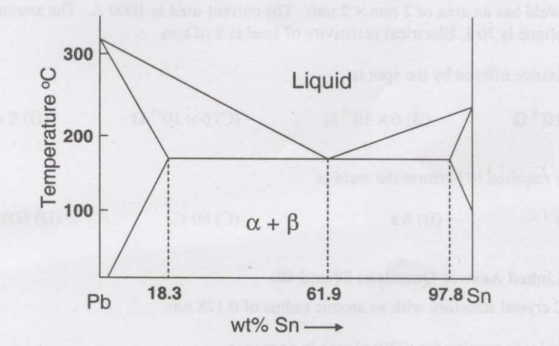
\includegraphics[width=0.5\textwidth]{figs/Q.53.png}
    \caption\centering{Pb-Sn PHASE DIAGRAM AT ATMOSPHERIC PRESSURE }
     \label{fig:placeholder}
\end{figure}
\item    A Pb-Sn hypo-eutectic alloy is slowly cooled from the liquid state to room temperature. The composition of the alloy whose microstructure consists of $25 wt\%$ lamellar constituent is
\hfill{\brak{\text{GATE MT 2009}}}
\begin {multicols}{2}
\begin{enumerate}
\item   $Pb - 29.2 wt\% \;Sn$
\item  $Pb - 35.5 wt\% \;Sn$
\item   $Pb-40.8 wt \% \;Sn$
\item  $Pb -61.9 wt\% \;Sn$
\end{enumerate}
\end{multicols}

\item   The minimum and maximum degrees of freedom in the above binary system are
\hfill{\brak{\text{GATE MT 2009}}}

\begin {multicols}{4}
\begin{enumerate}
\item  $1$ and $3$
\item   $0$ and $3$
\item  $1$ and $2$
\item  $0$ and $2$
\end{enumerate}
\end{multicols}
\subsection*{Common Data for Questions 55 and 56:}
An operator in a steel plant wants to reduce the phosphorous level in steel by treating it with an appropriate slag. The equilibrium phosphorous distribution ratio between slag and liquid steel, i.e. (wt$\%$ of P in slag) / (wt$\%$ of P in steel) is $100$ for the chosen slag composition. Assume before the treatment, the steel contains $0.2 wt\%\;P$.
\item   If the operator treats $1000 kg$ of liquid steel with $100 kg$ of slag, the resulting phosphorous content in liquid steel will be
\hfill{\brak{\text{GATE MT 2009}}}

\begin {multicols}{4}
\begin{enumerate}
\item   $0.001 \%$
\item    $0.002\%$
\item  $0.010\%$
\item $0.018\%$
\end{enumerate}
\end{multicols}
\item    Instead, the operator treats the $1000kg$ of liquid steel with $50 kg$ of slag. Then, the processed slag is removed and another $50 kg$ of fresh slag is added. The resulting phosphorous content in steel will be

\hfill{\brak{\text{GATE MT 2009}}}

\begin {multicols}{4}
\begin{enumerate}
\item   $0.0015\%$
\item   $0.0030\%$
\item   $0.0055\%$
\item $0.0090\%$
\end{enumerate}
\end{multicols}
\section*{Linked Answer Questions}
\subsection*{Statement for Linked Answer Questions 57 and 58:}
In automobile industry, electrical resistance welding is used for spot welding steel panels, each of $1.5 mm$ thickness. The weld has an area of $2 mm \times 2 mm$. The current used is $1000 A$. The amount of heat required to melt this spot volume is $36 J$. Electrical resistivity of steel is $8 \micro \ohm cm$.
\item   The resistance offered by the spot is
\hfill{\brak{\text{GATE MT 2009}}}

\begin {multicols}{4}
\begin{enumerate}
\item  $6 \times10^{-8} \ohm$
\item   $6 \times10^{-5} \ohm$
\item  $6 \times10^{+5} \ohm$
\item$6 \times10^{+8} \ohm$
\end{enumerate}
\end{multicols}
\item   The time required to perform the weld is
\hfill{\brak{\text{GATE MT 2009}}}

\begin {multicols}{4}
\begin{enumerate}
\item  $0.6 s$
\item   $6s$
\item  $60 s$
\item $600 s$
\end{enumerate}
\end{multicols}
\subsection*{Statement for Linked Answer Questions 59 and 60:}
Copper has FCC crystal structure with an atomic radius of $0.128 nm.$
\item   The interplanar spacing for $(220)$ planes in copper is
\hfill{\brak{\text{GATE MT 2009}}}

\begin {multicols}{4}
\begin{enumerate}
\item  $0.064 nm$
\item   $0.128 nm$
\item   $0.181 nm$
\item $0.256 nm$
\end{enumerate}
\end{multicols}
\item   In an X-ray diffraction experiment, radiation of wavelength $0.154 nm$ is used. Assuming the order of reflection to be 1, the Bragg angle for the $(220)$ set of planes in copper will be

\hfill{\brak{\text{GATE MT 2009}}}

\begin {multicols}{4}
\begin{enumerate}
\item  $12.56\degree$
\item  $36.98\degree$
\item  $48.98\degree$
\item  $74.21\degree$
\end{enumerate}
\end{multicols}



\end{enumerate}
\section*{*END OF THE QUESTION PAPER*}
 
\end{document}
